\chapter{Background}

\section{Automatic Text Summarisation}

Automatic text summarisation can be approached in many different ways. Generally the aim is to produce a summary, defined as “a text that is produced from one or more texts, that conveys important information in the original text(s)”(Radef et al. 2002). Allahyari et al. (2017) define Automatic text summarisation as “the task of producing a concise and fluent summary while reserving key information content and overall meaning”. Automatic text summarisation has many forms as each summarisation task uses different types of source documents, representation of content, and reasoning in producing a summary. The many forms of automatic text summarisation are discussed in this section.

\subsection{Summary Characteristics}

The context of the summarisation task must be addressed in order to best perform automatic text summarisation. Spärck-Jones (1999) in her taxonomy writes: “It is important to recognize the role of context factors because the idea of a general-purpose summary is manifestly an ignis factus”. The three context factors she identifies are input factors, purpose factors, and output factors. Input factors are classification of the representation of input document(s) in terms of structure, genre, format, and unit. The purpose factors are the relationship between the source and the output of summarisation and are described as dealing with situation, audience, and use. The output factors define the form of output of summary and are largely driven by the input and purpose factors of the system.

\subsection{Types of Summaries}

Gambhir and Gupta (2017) as well as Orăsan (2019) present a recent taxonomy to classify types of summaries. These classifications are important to consider when selecting an existing summarization method for a specific task or when creating a new automatic summarisation method. 

\subsubsection{Single document and Multi-document Summarisation}

The input to a summarisation system can either be a single document or a set of multiple documents. Single document summarization addresses the content of a single document and produces a summary of that single document. Multi-document summarization considers content from multiple documents and produces a summary of the discussed topics across all given documents. 

Many of the techniques of single document summarisation can be used in multi-document summarisation. Goldstein et al. (2000) identifies that: the redundancy of information of topically-related documents is much greater than in a single document making anti-redundancy methods crucial, the compression ratio (i.e. summary length with respect to document set length) is much smaller adding more difficulty to summarisation as compression demand increases, as well as the increased amount of co-referencing in a set of multiple documents than single documents. Many recent approaches attempt to deal with these issues. Methods to handle these issues will be discussed in the Redundancy Reduction section in this chapter.

\subsubsection{Extractive and Abstractive Summarisation}

The output of an automatic summarisation is either extractive or abstractive. An extractive summary is created from a subset of sentences from the source document(s). The sentences selected are those that the summarisation method finds most salient in the original text, using a similarity or centrality metric. An abstractive summary uses semantic models to generate a new piece of text that covers the themes, concepts or terms of the examined document or documents. Abstractive summarization requires natural language processing to extract concepts from the source material and to create an abstract summary from concept and word semantic relationships. Extractive summarization is simpler than abstractive but is limited because not all information in a sentence might not relate for a summary.

\subsubsection{Generic and Query-focused Summaries}

The purpose of summarisation is either generic or query-focused. Generic summaries attempt to summarize the content of all the material in the document or documents. This is the most common form of summary and is often used with single document summarisation. Query-focused, also referred to as topic-focused or user-focused, provides a summarisation based on a described need. These are commonly used with multi-document summarisation as multiple documents often contain a variety of topics. In this form of automatic text summarization a query is used both for the retrieval of documents as well as for the generation of the summary. 

Personalised summaries are a type of user-focused summary. Personalised summaries aim to produce a tailored summary based on a model of the user. Díaz and Gervás (2007) personalised summaries of newswire texts using a model of user interests based on keywords, domain-specific factors and user feedback. Li, Liu and Zhao (2015) suggest an update summarisation system which considers the novelty of the sentence by adding novelty as a variable to traditional integer linear programming approaches of summarisation.

\subsubsection{Supervised and Unsupervised Automatic Summarization}

Another distinction of summarization methods is supervised and unsupervised methods. Supervised methods require training from a pre-labeled data set. Supervised methods use two class classification algorithms, trained on labeled data, for selection of important content in source documents. Unsupervised methods are able to generate summaries from only using the source documents, and can therefore operate on new documents without the need for training. Unsupervised summarisation identifies relevant sentences using a set of heuristic rules and uses those sentences to generate a summary.


\section{Tasks of Summarisation}

\subsection{Intermediate Representation}

\subsection{Sentence Scoring}

\subsection{Sentence Selection}

\section{Summarisation Methods}

\subsection{Topic Representation}

\subsection{Indicator Representation and Machine Learning}

\subsection{Comparison of Methods}

\section{Query focused Summarisation}



\section{Figures}
Graphs, pictures and other images should be included in your report as a numbered, captioned figure. An example is given in Figure \ref{veldis}.

%%%%%%%%%%%%%%%%%%%%%%%%%%%%%%%%%%%%%%%%
\begin{figure}[h]
      \centering
      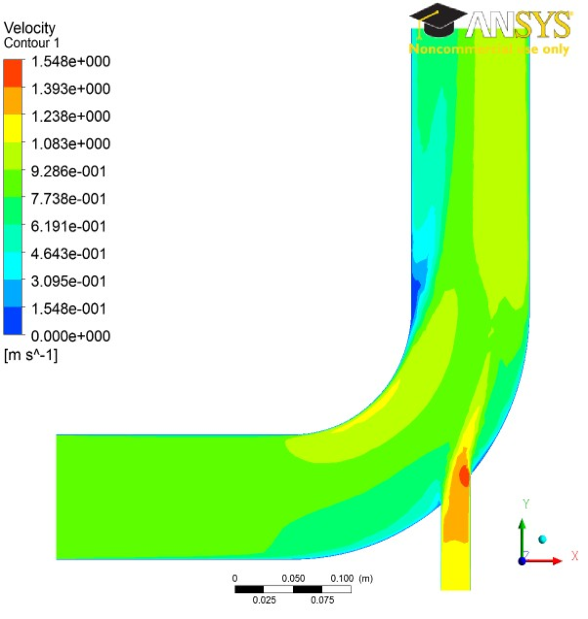
\includegraphics{background/5e1-1.pdf}
      \caption{Velocity distribution on the mid-plane for an inlet velocity for case 1.}
      \label{veldis}
\end{figure}
%%%%%%%%%%%%%%%%%%%%%%%%%%%%%%%%%%%%%%%%

The figure and caption should be centred. The figure numbering starts at 1 at the beginning of each chapter. The caption should provide a brief description of what is being shown. The figure should appear in the document after it is referred to in the text. No figure should be included which is not referred to in the text. Ensure that the size and resolution of images imported from software are sufficient to read any text.

\section{Tables}
Tables are an important way of displaying your results; Table \ref{tab:treatments} is a sample table, adapted from the Master/Doctoral Thesis template at \url{http://www.latextemplates.com/cat/theses}, which was generated with this code:

{\footnotesize
\begin{verbatim}
\begin{table}[b]
\caption{The effects of treatments X and Y on the four groups studied.}
\label{tab:treatments}
\centering
\begin{tabular}{l l l}
\toprule
\textbf{Groups} & \textbf{Treatment X} & \textbf{Treatment Y} \\\midrule
1 & 0.2 & 0.8\\
2 & 0.17 & 0.7\\
3 & 0.24 & 0.75\\
4 & 0.68 & 0.3\\
\bottomrule\\
\end{tabular}
\end{table}
\end{verbatim}
}

\begin{table}[b]
\caption{The effects of treatments X and Y on the four groups studied.}
\label{tab:treatments}
\centering
\begin{tabular}{l l l}
\toprule
\textbf{Groups} & \textbf{Treatment X} & \textbf{Treatment Y} \\
\midrule
1 & 0.2 & 0.8\\
2 & 0.17 & 0.7\\
3 & 0.24 & 0.75\\
4 & 0.68 & 0.3\\
\bottomrule\\
\end{tabular}
\end{table}

Tables are numbered in the same way as figures. Typically tables also have a short caption, but this is not universally true. The number and caption appear above the table, not below as with figures. Again, no table should appear in the report which has not been referred to in the text. Tables should come after they are discussed in the text. The exact formatting of the table depends somewhat on the content of the table, but in general, the text in the table should be the same font and size as the main text. 

\section{Equations}
All equations should be numbered sequentially. Do not restart the numbering at the beginning of each chapter. Unlike figures and tables, you may not need to refer to every equation in the text. You should take care to format equations properly. Do no simply try to use plain text. Use the equation layout facilities. An example of how equations should appear is shown in Equation \ref{sampleequation}. Here is the code for it:

{\footnotesize
\begin{verbatim}
\begin{equation}
\textrm{div}(\underline{u}) = \frac{\delta u}{\delta x} + \frac{\delta v}{\delta y} +
        \frac{\delta w}{\delta z} = 0
\label{sampleequation}
\end{equation} 
\end{verbatim}
}

\begin{equation}
\textrm{div}(\underline{u}) = \frac{\delta u}{\delta x} + \frac{\delta v}{\delta y} + \frac{\delta w}{\delta z} = 0
\label{sampleequation}
\end{equation} 

\section{Referencing published work}
It is important to give appropriate credit to other people for the work that they have shared through publications. In fact, you must sign a declaration in your report stating that you understand the nature of plagiarism. As well as avoiding plagiarism, citing results or data from the literature can strengthen your argument, provide a favourable comparison for your results, or even demonstrate how superior your work is.

There are many styles to reference published work. For example, the parenthetical style (which is also called the Harvard style) uses the author and date of publication (e.g. ``Smith and Jones, 2001''). There is also the Vancouver (or the citation sequence) style, which is shown in this document. In the Vancouver style, the publications are cited using a bracket number which refers to the list in the References section at the end of the report. The references are listed in order that they are cited in the report. A variant is name sequence style in which the publications are referenced by number, but the list is arranged alphabetically. For example, the text might say: several studies have examined the sound field around tandem cylinders generated by flow\cite{fitzpatrick2003flow,finnegan2010experimental}, while other investigations have focused on the effect of an applied sound field on the flow\cite{hall2003vortex}. Papers from conference proceedings\cite{jordan2001array}, books\cite{paidoussis2010fluid} and technical reports\cite{reyes2007power,iea2011} can be dealt with in the same style.

The Vancouver style has the advantage that it is a little more compact in the text and does not distract from the flow of the sentence if there are a lot of citations. However, it has the disadvantage that it is not immediately clear to the reader what particular work has been referenced.

It actually does not matter which particular referencing style is used as long as three important considerations are observed:
\begin{itemize}
\item the referencing style used throughout the document is consistent;
\item all material used or discussed in the text is properly cited;
\item nothing is included in the reference list that has not been cited.
\end{itemize}

This template has a suitable referencing style already set up -- you should use it and use the built-in BibTeX system to manage your references. See above for examples of how to cite a reference and look in the \texttt{sample.bib} file to see BibTeX references. Remember \href{http://scholar.google.com}{Google Scholar} and other search engines will give you BibTeX references for lots of academic publications. Otherwise, you can easily make up your own based on the examples in that file.